\documentclass[11pt]{llncs}
\usepackage{pbox,amssymb,amsmath,graphicx,color,multicol,mycommands}
\usepackage{amsfonts}
\usepackage{algorithm,url}
\usepackage[noend]{algpseudocode}
\usepackage{epsfig,latexsym,graphicx}

\newcommand{\bbR}{{\mathbb R}}
\newcommand{\bbZ}{{\mathbb Z}}
\newcommand{\bbS}{{\mathcal S}}
\newcommand{\bbK}{{\mathcal K}}
\newcommand{\bbV}{{\mathcal V}}
\newcommand{\bbI}{{\mathcal I}}
\newcommand{\bbC}{{\mathcal C}}
\newcommand{\bbL}{{\mathcal L}}
\newcommand{\remove}[1]{}
\setlength{\textwidth}{15.5cm}
\setlength{\textheight}{22cm}
\setlength{\oddsidemargin}{5pt}
\setlength{\evensidemargin}{5pt}
\setlength{\topmargin}{-0.05in}
\newtheorem{observation}{Observation}
\newtheorem{fact}{\noindent {\bf Fact}}

\begin{document}

\title{Modeling Mutagenicity Status of a Diverse Set of Chemical Compounds by Envelope Methods}
\author{Subho Majumdar}
\institute{Stat 8054 project summary\\School of Statistics,University of Minnesota- Twin Cities\\e-mail: majum010@umn.edu}
\maketitle

\begin{abstract}
We apply envelope methods on a dataset consisting of 508 diverse chemicals for two different purposes: estimating effects of the 307 predictors on mutagenicity of compounds, and employing discriminant analysis for the purpose of mutagenicity prediction. 'Two-deep' leave-one-out cross-validation is used for the purpose of prediction, meaning that envelope dimension of the predictive model is selected separately for each holdout compound. Rank deficiency in the data is tackled in two ways: by applying envelope methods as well as Supervised SVD on the first few principal components of the predictor matrix. Finally predictive performance of envelope models are compared with those of two earlier papers on the same dataset.\\

\textit{Keywords} : Envelope models; Supervised SVD; Dimension reduction; Two-deep cross-validation; Chemometrics; QSAR

\end{abstract}

\section{Introduction}
Envelope models \cite{cook} provide a flexible setup for dimension reduction in multivariate data analysis. They can work in conjunction with multivariate linear regression to produce estimates with reduced variance, and envelope-reduced data can also be used for class prediction by linear discriminant analysis. In this project we apply envelope methods on a Chemometrics dataset to assess their performance in estimation and prediction.

\paragraph{}Supervised Singular-Value Decomposition (SupSVD) is a recently proposed method \cite{supsvd} that provides a general framework, from which principal component analysis/ factor analysis and reduced-rank regression arise as special cases. In this a latent structure of a fixed dimension lower than the actual number of parameters is assumed and it is estimated using both the actual data and supervision data using a modified EM algorithm.

\paragraph{}Previous works on this dataset have focused on prediction through ridge regression models \cite{hawk} as well as variable selection through an iterative algorithm \cite{majum}. Here we shall use hierarchical envelope regression and SupSVD models for estimating the effects of the predictors on mutagenicity, as well as employ discriminant analysis on transformed data for the purpose of mutagenicity prediction.

\section{Data}
The data for this project were taken from the CRC Handbook of Identified Carcinogens and Non-carcinogens \cite{crc}. The response variable is 0/1 mutagen status obtained from \textit{Ames test of mutagenicity}. The 508 compounds- 256 mutagens and 252 non-mutagens were classified as mutagen (scored 1) if its Ames score exceeded a certain cutoff, non-mutagen (scored 0) otherwise. The chemical compounds in this dataset come from diverse chemical classes, for example, aliphatic alkanes, Monocyclic and polycyclic compounds and Amines.
\paragraph{}We have 4 types of descriptors for each chemical compound:
\begin{enumerate}
\item \textbf{Topostructural (TS)}- define the molecular topology, i.e. connectedness of atoms within a molecule (\textit{103 descriptors})
\item \textbf{Topochemical (TC)}- have information on atom and bond types (\textit{195 descriptors})
\item \textbf{3-dimensional (3D)}- define 3-dimensional aspects of the overall molecular structure (\textit{3 descriptors})
\item \textbf{Quantum-Chemical (QC)}- electronic aspects of molecular structure (\textit{6 descriptors})
\end{enumerate}

\section{Methods}
\subsection{Envelope regression model}
The basic structure of the model \cite{cook}, for $i = 1,2,...,n $, is
$$ \bfY_i = \bfalpha + \bfX_i\bfbeta + \bfepsilon_i,\quad \bfepsilon_i\sim \mathcal N_r(\bfZero,\bfSigma)$$
$$\mbox{ with }\bfSigma = \bfGamma\bfOmega\bfGamma^T + \bfGamma_0\bfOmega_0\bfGamma^T$$
where $\bfY\in\BR^{n\times r}$ multivariate response vector, $\bfX\in\BR^{n\times p}$ non-stochastic predictors $\bfalpha\in\BR^r$ is the intercept and $\bfbeta\in\BR^{r\times p}$ the matrix of regression coefficients, both being unknown. Finally $\bfGamma\in\BR^{r\times u},\bfGamma_0\in\BR^{r\times (r-u)}$ are the semi-orthogonal basis matrices of $\cE_\bfSigma(\cB)$ and its orthogonal complement, respectively, with $\cB = \mbox{span}(\bfbeta)$ and $0\leq u\leq r$ being the dimension of the envelope. Also $\bfOmega = \bfGamma\bfSigma\bfGamma^T, \bfOmega_0 = \bfGamma_0\bfSigma\bfGamma_0^T$ are the coordinate matrices corresponding to $\bfGamma, \bfGamma_0$.
\paragraph{}For estimation purposes, we use the 0/1 mutagenicity status as univariate predictor and the data on 307 descriptors as multivariate responses.

\subsection{Supervised Singular-Value Decomposition (SupSVD)}
This recently proposed model \cite{supsvd} assumes a latent lower-dimensional structure for the matrix of predictors $\bfX\in\BR^{n\times p}$ and estimates it using a supervision data matrix $\bfY\in\BR^{n\times r}$. The assumed model is:
$$ \bfX = \bfY\bfB\bfV^T + \bfF\bfV^T + \bfE $$
where $\bfB\in\mathbb{R}^{r\times q}$ is the multivariate matrix of coefficients, $\bfV\in\mathbb{R}^{p\times q}$ full-rank loading matrix. Here $0\leq q\leq r$ is the dimension of the underlying space of latent parameters, and $\bfF\sim\mathcal{N}_q(\bf0,\bfSigma_f), \bfE\sim\mathcal{N}_p(\bf0,\sigma_e^2\bfI_p)$ are random error matrices ($\bfSigma_f\in\mathbb{R}^{q\times q}$ diagonal). Hence the overall covariance matrix $\bfSigma\in\mathbb{R}^{p\times p}$ can be decomposed as $\bfSigma = \bfV\bfSigma_f\bfV^T + \sigma_e^2\bfI_p$. The modified EM algorithm to obtain the unknown parameters $\bftheta=(\bfB,\bfV,\bfSigma_f,\sigma_e^2)$ is given in the appendix.

\paragraph{}The vector of mutagenicity status is now used as the supervision data matrix $\bfY$, while the data on 308 predictors is the matrix $\bfX$ (notice that $\bfX$ and $\bfY$ are reversed from 3.1). The structure of the envelope model might seem similar to the SupSVD model considering the facts that both of them consider decompositions of the sample covariance matrix $\bfSigma$, but they arise from different underlying assumptions. While envelope models try to obtain the smallest reducing subspace of $\bfSigma$ that contains the matrix of coefficients $\bfB$, SupSVD can be seen as a generalization of the factor analysis/ PCA model, in which the data matrix itself is a result of a transformation on the underlying space of unknown independent predictors.

\subsection{Tackling rank-deficiency} Because of the rank-deficient nature of the original data envelope methods cannot be applied to the actual variables. Instead we first do Principal Component Analysis on the matrix of predictors $\bfY$, take the minimum number of PCs ($k$) that explain $\geq 90\%$ of the total variance in a loading matrix $\bfL\in\BR^{r\times k}$ and apply the methods in 3.1 on the transformed predictors $\bfL^T\bfY$ instead of $\bfY$. Due to the substantially less computational burden of the SupSVD algorithm, both the 90\% and 95\% cutoffs from PCA were considered as the dimension of the space of latent predictors i.e. $q$.

\subsection{Linear Discriminant Analysis} To assess the predictive performance of envelope models, we first estimate the envelope basis as per 3.1, say $\hat\bfGamma$, reduce the matrix of predictors by multiplying it with the basis and then apply Fisher's Linear Discriminant Analysis \cite{fish} on $\hat\bfGamma^T\bfY$.

\paragraph{}For SupSVD the notations are reversed and $\bfX$ is our $508\times 307$ data matrix. After obtaining the loading matrix $\bfV$, we transform the data matrix as: $\bfU = \bfX\bfV$, and apply LDA on $\bfU$, taking $\bfY$ as the 0/1 class variable.

\section{Results}
\subsection{Envelope estimation}
All envelope analyses were done on MATLAB version R2010a \cite{matlab}. A hierarchical approach is taken for building the model, first using only TS and TC descriptors to build envelope models, then using TS+TC and finally the full set of descriptors. To take care of the difference in magnitude across predictors, each entry $x$ in the data matrix $\bfX$ is transformed as: $x\mapsto\log(x+C)$, where $C=-\lfloor x\rfloor$ if $x<0$. and $C=1$ otherwise. After this we standardize $\bfX$ and $\bfY$.

\paragraph{}For the envelope regression model, we get back the original coefficient estimates and their standard errors by back-transformation on their principal components counterparts. If $\bfb\in\BR^k$ is the envelope estimate of coefficients of $k$ principal components and $\hat\nu_1,...,\hat\nu_k$ their standard errors, then $\bfL\bfb$ gives coefficient estimates in the original scale, and $\sum_{i=1}^k l_{ji}^2\hat\nu_i^2$ the variance of the $j^{th}$ coefficient, with $j=1,2,...,r$.

\paragraph{}The first 3 models in \textbf{Table 1} show significant gains due to envelopes, especially for the first 2 principal components. For the full set of predictors, the iterative algorithm did not converge for the default tolerance values of the objective and gradient functions, and the results here are from a model obtained with higher tolerance values.

\paragraph{}Significance of individual predictors were obtained for each model by $t$-ratios. For the single variable-type models, linearly correlated predictors tend to be simultaneously significant, but this behavior is is less observed in the combined model (TS+TC) (\textbf{Table 2}).

\begin{table*}[t]\centering
    \begin{tabular}{|c|c|c||c|c|c|c|c|c|}\hline
    \textbf{Set of} & \textbf{No. of} & \textbf{Envelope} &	\multicolumn{3}{c|}{\textbf{\% var explained by}}	& \multicolumn{3}{c|}{\textbf{Envelope gain ratios for}}\\\cline{4-9}
    \textbf{descriptors}                  & \textbf{PCs}                                                 & \textbf{dim} ($u$) & \hspace{.2cm}\textbf{PC1}\hspace{.2cm}	& \hspace{.2cm}\textbf{PC2}\hspace{.2cm}   & \hspace{.2cm}\textbf{PC3}\hspace{.2cm}  & \hspace{.2cm}\textbf{PC1}\hspace{.2cm}	& \hspace{.2cm}\textbf{PC2}\hspace{.2cm}   & \hspace{.2cm}\textbf{PC3}\hspace{.2cm}  \\\hline\hline
    \textbf{TS}                 & 7                                                 & 3                        & 70.43 & 10.35 & 2.60 & 25.91              & 36.17 & 2.10 \\ \hline
    \textbf{TC}                 & 8                                                 & 4                        & 75.89 & 6.52  & 2.42 & 15.40              & 35.26 & 1.00 \\\hline
    \textbf{TS + TC}            & 13                                                & 6                        & 70.27 & 7.94  & 2.21 & 10.40              & 37.99 & 1.22 \\\hline
    \textbf{Full} & 15 & 11 & 58.19 & 7.60 & 5.98 & 1.00 & 1.00 & 1.00 \\\hline
    \end{tabular}
    \caption{Summary of envelope models for different sets of descriptors}
\end{table*}

\begin{table}[ht]\centering
    \begin{tabular}{|c|c|c|c|}\hline
    \textbf{Set of}      & \multicolumn{2}{c|}{\textbf{No. of descriptors}} & \textbf{Significant}\\\cline{2-3}
    \textbf{descriptors} & \hspace{.1cm}\textbf{Total}\hspace{.1cm}              & \textbf{Significant} & \textbf{PCs}\\\hline\hline
    TS          & 103                & 51         & 4, 5, 7 \\\hline
    TC          & 195                & 98         & 1, 3, 8\\\hline
    TS + TC     & 298                & 89         & 4, 7, 11\\\hline
    Full        & 307                & 56         &  2, 3, 8, 10, 14\\\hline
    \end{tabular}
    \caption{Significance of predictors in envelope models}
\end{table}

\begin{table}[H]\centering
    \begin{tabular}{|c|c|c|}
    \hline
    \textbf{Case}      & \multicolumn{2}{c|}{\textbf{Mean error(SE)}}              \\ \cline{2-3}
             & \textbf{SupSVD}         & \textbf{PCA}            \\ \hline\hline
    \hspace{.2cm}\textbf{I. SupSVD}\hspace{.2cm} & \hspace{.2cm}0.0768 (0.034)\hspace{.2cm} & \hspace{.2cm}0.0794 (0.031)\hspace{.2cm} \\ \hline
    \textbf{II. PCA}   & 0.0803 (0.032) & 0.0768 (0.034) \\ \hline
    \end{tabular}
    \caption{$MSE_\bfV$ means and standard errors for the two simulation scenarios}
\end{table}

\subsection{SupSVD analysis}The efficacy of this method in estimation of the loading matrix $\bfV$ in the supervised setup is demonstrated by the following simulation. We set $n=1000,p=10,r=2,q=3$. We generate the entries of the $1000\times 2$ matrix $\bfY$ as iid Ber$(1,0.5)$. The loading matrix $\bfV$ is obtained by taking $p$ iid samples from $\mathcal{N}_r(\bf0,\bfI_r)$ and orthogonalizing the columns. Finally we take $\bfSigma_f=$diag$(10,7,4),\sigma_e^2=2$, and generate $\bfF,\bfE$. We choose $\bfB$ to for two scenarios:
\begin{enumerate}
\item $r$ rows of $\bfB$ as iid samples from $\mathcal{N}_q(\bf0,\bfI_q)$. Thus $ \bfX = \bfY\bfB\bfV^T + \bfF\bfV^T + \bfE $ and this is the typical SupSVD scenario.
\item Take $\bfB=\bf0$. Then we have $ \bfX = \bfF\bfV^T + \bfE $ and the model becomes an unsupervised factor analysis/PCA model.
\end{enumerate}
For each of the two cases, we generate 1000 samples and apply SupSVD and PCA on each of them. The error in estimating $\bfV$ can be calculated for both the methods:
$$ MSE_{\bfV} = \frac{1}{pq}\Vert\bfV-\hat\bfV\Vert^2_\mathbb{F} $$
For PCA, $\hat\bfV$ is taken as the first $q$ columns of the original PCA loading matrix obtained. The results are summarized in \textbf{Table 3}. In presence of supervision data, SupSVD turns out to be more accurate than unsupervised PCA, but this is not the case when $\bfB=\bf0$.

\paragraph{}For each of the 4 subsets of the data: TS, TC, TS+TC and full, we did PCA on the data and take the first few components that explain 90\% (or 95\%) of the total variance, take the number of components as the underlying dimension and perform the SupSVD analysis. The diagonal entries of the matrix $\bfSigma_f$ lists the variance of the latent components. These can be compared to variances of the same principal components of the data to study the effect due to predictors. For example, \textbf{Table 4} lists the top 8 PC's that explain 95\% of the total variances in the TS data, and compares it to the diagonal entries of the $\bfSigma_f$ obtained.

\subsection{Predictive performance of models} Prediction using envelope LDA was done by leave-one-out cross-validation. While doing cross-validation here it is imperative not to fix the dimension of the envelope $u$ beforehand and then take holdout samples to build envelope models. Since information from the holdout compound has already been used to obtain $u$, this overestimates the predictive power of the method (hence called Na\"{i}ve CV, see \textbf{Figure 1}). Instead in each step one should first separate the holdout sample, then use other samples to predict the envelope dimension ($u$) each time and use that $u$ to build predictive model for that holdout sample. Since we are aiming for prediction, one should select the envelope dimension each time by CV as well (Two-fold CV), but due to larger computational burden we select it by AIC/BIC each time.

\paragraph{}\textbf{Table 5} summarizes the predictive performance of all the methods (for SupSVD, numbers in brackets indicate dimension of the latent variable space). Envelope reduction after transformation by first few principal components seems to perform the worst in terms of prediction. SupSVD performs better, and for a larger number of latent components prediction performance is slightly better, but it still can't beat previous analyses.

\begin{table}[t]\centering
    \begin{tabular}{|c|c|c|c|c|c|c|c|c|}
    \hline
    \#\textbf{Component} &  1       & 2     & 3    & 4     & 5     & 6     & 7     & 8     \\ \hline
    \textbf{Before}       & \hspace{.2cm}75.425\hspace{.2cm} & \hspace{.2cm}8.247\hspace{.2cm} & \hspace{.2cm}5.01\hspace{.2cm} & \hspace{.2cm}3.135\hspace{.2cm} & \hspace{.2cm}2.642\hspace{.2cm} & \hspace{.2cm}1.366\hspace{.2cm} & \hspace{.2cm}1.159\hspace{.2cm} & \hspace{.2cm}0.908\hspace{.2cm} \\\hline
    \textbf{After}        & 75.186 & 8.187 & 4.922 & 2.992 & 2.476 & 1.303  & 1.108 & 0.856 \\ \hline
    \end{tabular}
    \caption{First 8 components of TS data, before and after SupSVD}
\end{table}

\begin{figure}[t]
\begin{center}
   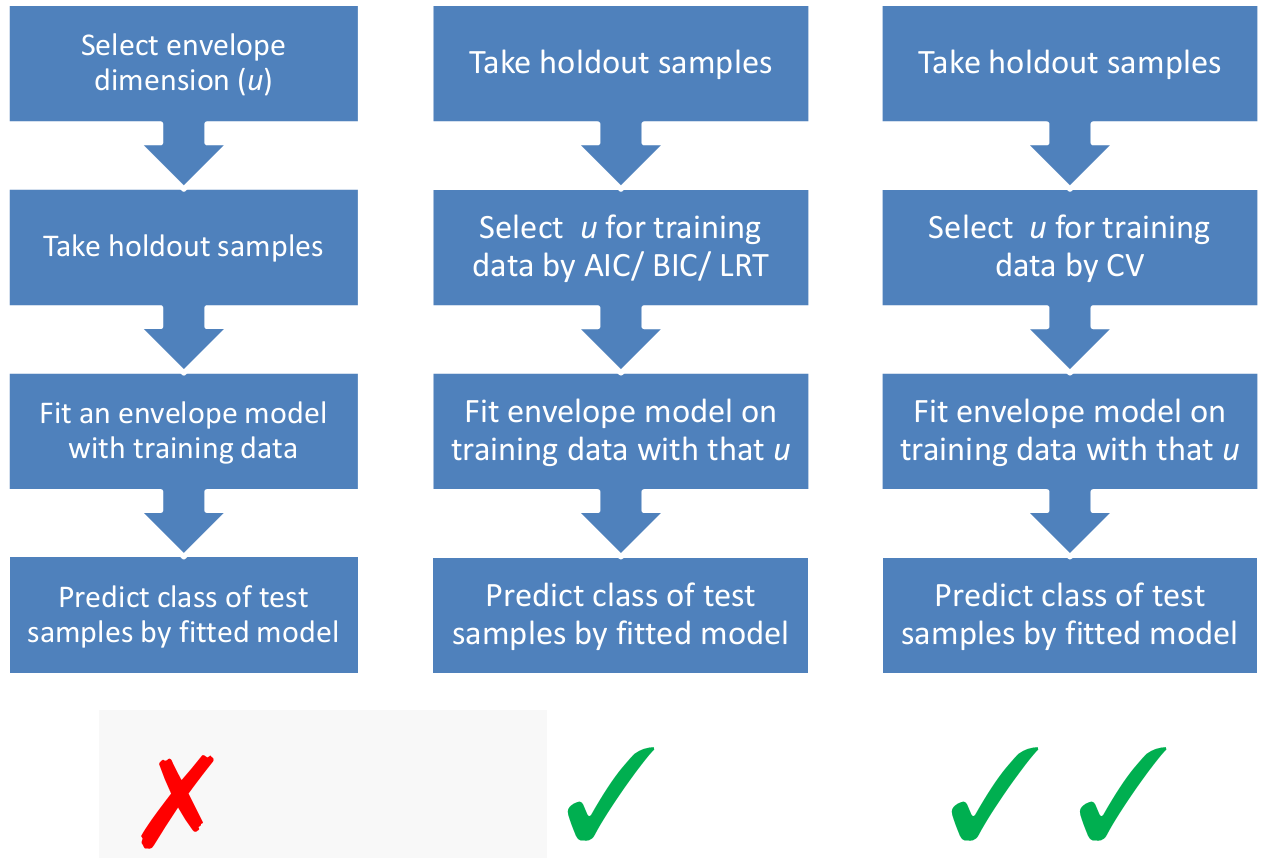
\includegraphics[height=7cm]{cv.png}
   \label{fig:fig1}
   \caption{Na\"{i}ve CV vs. Two-fold CV}
\end{center}
\end{figure}

\begin{table}[t]\centering
    \begin{tabular}{|c|c|c|c|c|c|}
    \hline
    \textbf{Model}                                     & \textbf{Type of predictors} & \textbf{No. of}     & \multicolumn{3}{c|}{\textbf{Correct classification} \%}\\\cline{4-6}
    \textbf{description}                               & \textbf{in model}           & \textbf{predictors} & \quad\textbf{Total}  \quad                   & \textbf{Mutagens} & \textbf{Non-mutagens} \\ \hline
    Ridge regression\cite{hawk}                          & TS+TC              & 298        & 76.97                     & 83.98    & 69.84        \\ \hline
    Ridge regression\cite{hawk}                          & TS+TC+3D+QC        & 307        & 77.17                     & 84.38    & 69.84        \\ \hline
    \pbox{10cm}{Ridge regression after \\variable selection\cite{majum}} & TS+TC+AP           & 203        & 78.35                     & 84.38    & 72.22        \\ \hline\hline
                                  & TS                 & 103        & 57.09                     & 65.63    & 48.41        \\\cline{2-6}
    Envelope LDA                                         & TC                 & 195        & 58.27                     & 69.92    & 46.43        \\\cline{2-6}
    ~                                         & TS+TC              & 298          & 60.24 & 69.14        & 51.19            \\ \hline\hline
     & TS & 103 (5) & 59.45 & 70.31 & 48.41 \\\cline{2-6}
  SupSVD LDA   & TC & 195 (37) & 70.47 & 76.56 & 64.29 \\\cline{2-6}
  90\% cutoff  & TS+TC & 298 (32) & 68.90 & 75.39 & 62.30 \\\cline{2-6}
    & TS+TC+3D+QC & 307 (34) & 70.47 & 77.73 & 63.09 \\\hline\hline
    
     & TS & 103 (8) & 60.04 & 67.58 & 52.38 \\\cline{2-6}
  SupSVD LDA & TC & 195 (51) & 72.44 & 78.13 & 66.67 \\\cline{2-6}
  95\% cutoff  & TS+TC & 298 (48) & 70.47 & 78.91 & 61.90 \\\cline{2-6}
    & TS+TC+3D+QC & 307 (51) & 71.06 & 78.91 & 63.09 \\\hline
    \end{tabular}
    \caption{Prediction performance of various models}
\end{table}

%\begin{table}[!h]
%\begin{center}
%\begin{tabular}[c]{|c|c||c|c|c|c|c|c|c|}\hline
% & & \multicolumn{7}{c|}{Method of analysis (powers in percentage)}\\\cline{3-9}
%\begin{large} $p$ \end{large} &\begin{large} $d$ \end{large} & All & All & Omit affected & Omit treated & Treatment & Constant & Non-parametric \\
% & (mm Hg) & underlying & observed & subjects & subjects & as covariate & adjustment & adjustment\\\hline\hline
% & 10 & 44.7 & 42.4 & 29.9 & 31.7 & 29.0 & 44.3 & 41.7\\\cline{2-9}
% & 15 & 81.2 & 79.1 & 60.8 & 68.6 & 59.5 & 80.9 & 79.8\\\cline{2-9}
%\begin{large} \textbf{0.1} \end{large} & 20 & 97.3 & 97.0 & 86.1 & 89.9 & 85.9 & 97.3 & 97.1\\\cline{2-9}
% & 25 & 99.7 & 99.7 & 97.5 & 98.1 & 97.0 & 99.7 & 99.7\\\cline{2-9}
% & 30 & 100.0 & 100.0 & 99.7 & 99.7 & 99.5 & 100.0 & 100.0\\\cline{2-9}\hline\hline
%
% & 10 & 80.3 & 79.1 & 53.3 & 65.9 & 56.6 & 80.0 & 78.0\\\cline{2-9}
% & 15 & 98.9 & 97.8 & 90.2 & 93.9 & 91.6 & 98.6 & 98.8\\\cline{2-9}
%\begin{large} \textbf{0.3} \end{large} & 20 & 100.0 & 100.0 & 99.3 & 99.8 & 99.7 & 100.0 & 100.0\\\cline{2-9}
% & 25 & 100.0 & 100.0 & 100.0 & 100.0 & 100.0 & 100.0 & 100.0\\\cline{2-9}
% & 30 & 100.0 & 100.0 & 100.0 & 100.0 & 100.0 & 100.0 & 100.0\\\cline{2-9}\hline\hline
%
% & 10 & 86.0 & 84.3 & 65.5 & 74.0 & 70.4 & 86.0 & 83.2\\\cline{2-9}
% & 15 & 99.7 & 98.8 & 95.2 & 97.6 & 96.9 & 99.7 & 99.5\\\cline{2-9}
%\begin{large} \textbf{0.5} \end{large} & 20 & 100.0 & 100.0 & 99.9 & 100.0 & 100.0 & 100.0 & 100.0\\\cline{2-9}
% & 25 & 100.0 & 100.0 & 100.0 & 100.0 & 100.0 & 100.0 & 100.0\\\cline{2-9}
% & 30 & 100.0 & 100.0 & 100.0 & 100.0 & 100.0 & 100.0 & 100.0\\\cline{2-9}\hline
%\end{tabular}
%\caption{Powers obtained by different methods for $\delta' = 1$}
%\end{center}
%\end{table}

\section{Conclusion}
Looking at the scatterplot of points for the first 5 latent components in the data on TS variables only (see Appendix 2), we can see that a linear approach to discriminant analysis for this data might not be a good idea itself. Here the efficacy of envelope methods has been demonstrated for estimation purposes, its performance in prediction is not good. Possible reasons for this are high ratio of material to immaterial variation, heteroskedasticity caused by diverse chemical classes among compounds and variation of scales between different types of variables. A more detailed formulation of the envelope model keeping these issues in mind should improve the predictive performance. Also, a logistic envelope regression model could be a new approach towards estimation and prediction. Finally, the supervised SVD has the potential to be a plausible approach towards classification and supervised data analysis because of its general framework and more computational stability compared to envelopes.

\section*{Acknowledgment}I thank Profs. Dennis Cook and Adam Rothman for their guidance and valuable inputs throughout the project and Xin Zhang for sharing his MATLAB codes for logistic envelope analysis.

\bibliographystyle{acm}
\bibliography{envchemo}

\section*{Appendix 1: Algorithm for SupSVD parameter estimation}
We start with the model as defined in 3.2, and our goal is to estimate the parameter $\bftheta=(\bfB,\bfV,\bfSigma_f,\sigma_e^2)$. Define $\bfU=\bfY\bfB+\bfF$. Then using the following Expectation-Maximization-Standardization (EMS) algorithm one can obtain the parameter estimates iteratively (as described in \cite{supsvd}). It is proved that the likelihood function $\mathcal L(\bfX|\bftheta)$ increases in each iteration, hence in the stopping criterion we subtract the likelihood function of the current iterate from the one of the next iterate.

\begin{algorithm}
\caption{The EMS Algorithm for Parameter Estimation under the SupSVD Model}
\begin{algorithmic}[1]
\Procedure{SupSVD}{data $\bfX\in\mathbb{R}^{n\times p}$, supervision data $\bfY\in\mathbb{R}^{n\times r}$}
\State Set initial values for the parameters $\bftheta^{(0)} = (\bfB^{(0)},\bfV^{(0)},\bfSigma_f^{(0)},\sigma_e^{2(0)}); i=0$
\While {$\mathcal{L}(\bfX|\bftheta^{(i+1)})-\mathcal{L}(\bfX|\bftheta^{(i)})>$threshold}
\vspace{.2cm}
\State \textbf{E step}: Calculate
\State \hspace{.5cm}E$_{\bfU} (\bfU|\bfX,\bftheta^{(i)}) = \bfTheta_{\bfU|\bfX}^{(i)} = \left[\bfY\bfB^{(i)}\left(\sigma_e^{2(i)}\bfSigma_f^{(i)^{-1}}\right)+\bfX\bfV^{(i)}\right]\left[\bfI_q+\sigma_e^{2(i)}\bfSigma_f^{(i)^{-1}}\right]^{-1}$
\State \hspace{.5cm}Var$_{\bfU} (\bfU|\bfX,\bftheta^{(i)}) = \bfOmega_{\bfU|\bfX}^{(i)} = \left[\bfSigma_f^{(i)^{-1}}+\sigma_e^{-2(i)}\bfI_q\right]^{-1}$
\vspace{.2cm}
\State \textbf{M step}: Calculate unconstrained maximizers
\State \hspace{.5cm}$\hat\bfB = (\bfY^T\bfY)^{-1}\bfY^T\bfTheta_{\bfU|\bfX}^{(i)}$
\State \hspace{.5cm}$\hat\bfV = \bfX^T\bfTheta_{\bfU|\bfX}^{(i)}\left[n\bfOmega_{\bfU|\bfX}^{(i)} + \bfTheta_{\bfU|\bfX}^{(i)T}\bfTheta_{\bfU|\bfX}^{(i)}\right]^{-1} $
\State \hspace{.5cm}$\widehat{\bfSigma_f} = \frac{1}{n}\left[n\bfOmega_{\bfU|\bfX}^{(i)} + \bfTheta_{\bfU|\bfX}^{(i)T}\bfTheta_{\bfU|\bfX}^{(i)} + \hat\bfB^T\bfY^T\bfY\hat\bfB - \hat\bfB^T\hat\bfY^T\bfTheta_{\bfU|\bfX}^{(i)} - \bfTheta_{\bfU|\bfX}^{(i)T}\bfY\hat\bfB\right]$
\State \hspace{.5cm}$\widehat{\sigma_e^2} = \frac{1}{np}\left[\tr(\bfX^T\bfX) + 2\tr\left(\bfTheta_{\bfU|\bfX}^{(i)}\hat\bfV^T\bfX^T\right) + n\tr\left(\hat\bfV^T\hat\bfV\bfOmega_{\bfU|\bfX}^{(i)}\right) + \tr\left(\bfTheta_{\bfU|\bfX}^{(i)}\hat\bfV^T\bfV\bfTheta_{\bfU|\bfX}^{(i)T}\right)\right]$
\vspace{.2cm}
\State \textbf{S step}: Calculate next iterates
\State \hspace{.5cm}Get $\bfV^{(i+1)},\bfSigma_f^{(i+1)}$ from eigen-decomposition of $\hat\bfV\widehat{\bfSigma_f}\hat\bfV^T$: $\bfV^{(i+1)}\bfSigma_f^{(i+1)}\bfV^{(i+1)T} = \hat\bfV\widehat{\bfSigma_f}\hat\bfV^T$
\State \hspace{.5cm}Reorder columns of $\bfV^{(i+1)}$, rows/columns of $\bfSigma_f^{(i+1)}$ as per decreasing column norm of $\bfX\bfV^{(i+1)}$
\State \hspace{.5cm}$\bfB^{(i+1)} = \hat\bfB\hat\bfV^T\bfV^{(i+1)}$
\State \hspace{.5cm}$\sigma_e^{2(i+1)} = \widehat{\sigma_e^2}$
\vspace{.2cm}
\State Set $i\leftarrow i+1$
\EndWhile
\State \textbf{end while}
\EndProcedure
\end{algorithmic}
\end{algorithm}

\newpage\section*{Appendix 2: Scatterplot of latent components}
\begin{figure}[H]
\begin{center}
   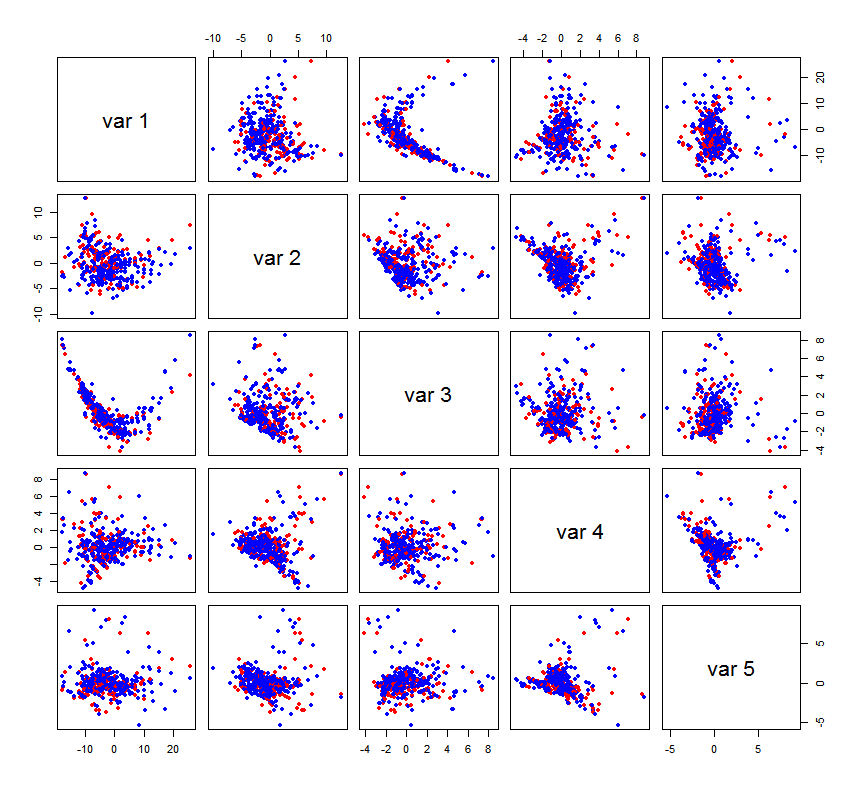
\includegraphics[height=15cm]{pcplot.png}
   \label{fig:fig1}
   \caption{Plot of first 5 latent components for TS data, 90\% cutoff (red = mutagen, blue = non-mutagen)}
\end{center}
\end{figure}
\end{document} 
